\documentclass[informe]{tesis-usach}

\usepackage{tikz}
\usetikzlibrary{arrows, calc, decorations.markings, math, arrows}
\usetikzlibrary{matrix, chains, positioning, decorations.pathreplacing, shapes, snakes}
\usepackage{pgfplots}

\usepackage{pgfgantt}

\title{Análisis de la convergencia del algoritmo {\em simulated annealing} para redes neuronales profundas}
\informe{Propuesta de tesis}
\facultad{Facultad de Ingeniería}
\departamento{Departamento de ingeniería informática}
\author{Felipe Alberto Reyes González}
\programa{Magíster en Ingeniería Informática}
\profesor{Victor Parada}
\celular{890 26 317}
\correo{felipe.reyesg@usach.cl}
\date{\today}

\usepackage{amsmath}
% TIPOS DE ENTRADAS : http://newton.ex.ac.uk/tex/pack/bibtex/btxdoc/node6.html
% CAMPOS : http://newton.ex.ac.uk/tex/pack/bibtex/btxdoc/node7.html
\begin{document}
\renewcommand{\contentsname}{Tabla de contenido}
\renewcommand{\refname}{Bibliografía}
\renewcommand{\appendixname}{Apéndice}
\renewcommand{\appendixtocname}{Apéndices}
\renewcommand{\appendixpagename}{Apéndices}
\renewcommand{\tablename}{Tabla}

% helvetica en el cuerpo del documento
% \sffamily

% \frontmatter
\maketitle
% \aditionalpages
% \indice
% \mainmatter

%%%%%%%%%%%%%%%%%%%%%%%%%%%%
% Inicio cosas importante
%%%%%%%%%%%%%%%%%%%%%%%%%%%%
%
\tableofcontents
\newpage

\section{Descripción del problema}
%\subsection{Las redes neuronales}
El elemento básico de las redes neuronales ({\em Neural Networks}, NN) es el nodo, que recibe un vector de entrada para producir una salida. Cada entrada tiene asociado un vector de pesos $w$, que se va modificando durante el proceso de aprendizaje. Cada unidad aplica una función $f$ sobre la suma ponderada de las entradas ponderada
%\begin{eqnarray}
%	$$ y_{i} = \sum_{j} w_{ij}y_{j}\label{eq:entrada} $$
%\end{eqnarray}
donde el resultado puede servir como entrada de otras unidades.

Existen dos fases importante dentro del modelo
\begin{itemize}
	\item Fase de entrenamiento: Se usa un conjunto de datos o patrones de entrenamiento para determinar los pesos que definen el modelo de la NN. Se calculan de manera iterativa, de acuerdo con los valores de entrenamiento, con el objeto de minimizar el error cometido entre la salida obtenida por la NN y la salida deseada.

	\item Fase de prueba: Durante el entrenamiento, el modelo se ajusta al conjunto de entrenamiento, perdiendo la habilidad de generalizar su aprendizaje a casos nuevos, a esta situación se le llama sobreajuste.
	Para evitar el sobreajuste, se utiliza un segundo grupo de datos diferentes, el conjunto de validación, que permitirá controlar el proceso de aprendizaje.
\end{itemize}
Los pesos óptimos se obtienen minimizando una función. Uno de los criterios utilizados es la minimización del error cuadrático medio entre el valor de salida y el valor real esperado.


\subsection{El perceptrón multicapa}
Dentro de las redes neuronales, el perceptrón multicapa es una de las arquitecturas más usadas para resolver problemas. Esto es debido a que poseen la capacidad de ser un aproximador universal \cite{Minsky1969b}. Esto no implica que sea una de las redes más potentes o con mejores resultados, el perceptrón multicapa posee una serie de limitaciones, como el proceso de aprendizaje para problemas que dependan de un gran número de variables, la dificultad para realizar un análisis teórico de la red debido a la presencia de componentes no lineales y a la alta conectividad.

\subsubsection{Arquitectura}
El perceptron multicapa posee una estructura de capas compuestas por neuronas. Cada una de las capas está formada por un conjunto de neuronas y se distinguen tres tipos de capas: la capa de entrada, las capas ocultas y la capa de salida.

\begin{imagen}
	\scalebox{0.8}{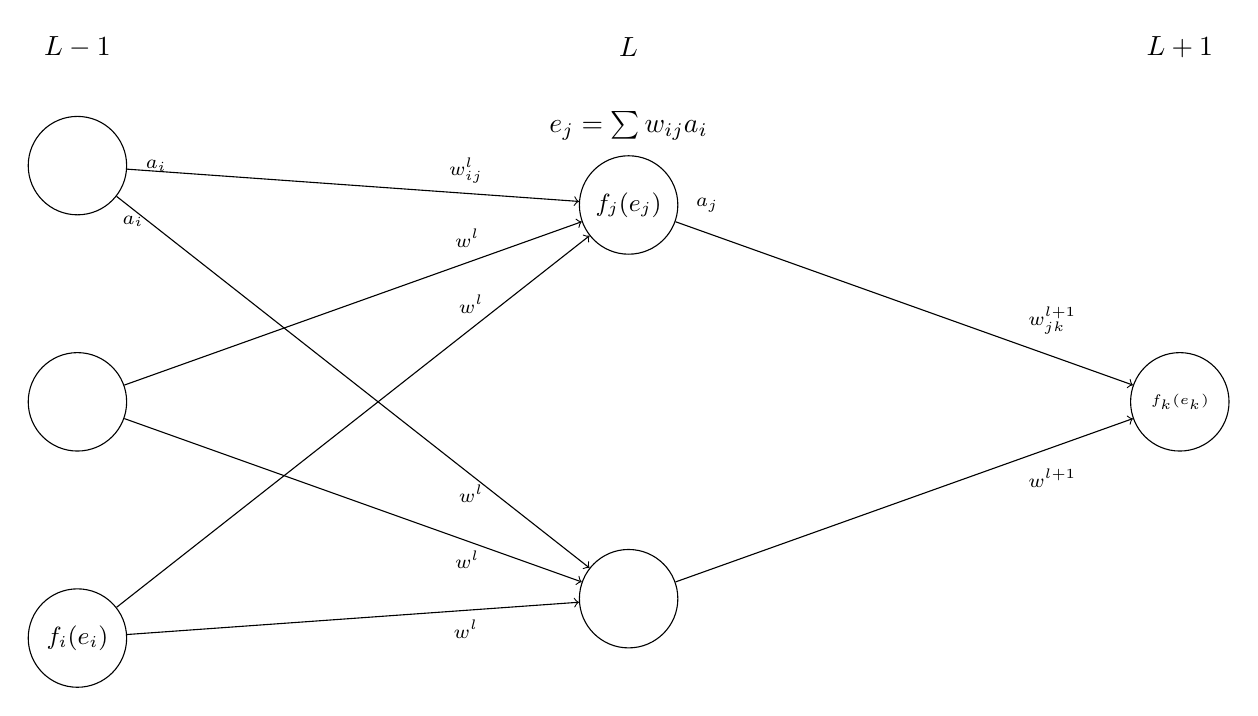
\begin{tikzpicture}

	\tikzstyle{nodo}=[circle, draw, minimum size=1.25cm]
	\tikzstyle{upw}=[dashed, red, ->, line width = 1pt]

	\coordinate (l_0) at (0, 4.5);
	\coordinate (l_1) at (7, 4.5);
	\coordinate (l_2) at (14, 4.5);

	\coordinate (f_1_1) at (0, 3); % CAPA ENTRADA
	\coordinate (f_1_2) at (0, 0); % CAPA ENTRADA
	\coordinate (f_1_3) at (0, -3); % CAPA ENTRADA
	\coordinate (f_2_1) at (7, 2.5); % CAPA OCULTA 1
	\coordinate (f_2_2) at (7, -2.5); % CAPA OCULTA 1
	\coordinate (f_3_1) at (14, 0); % CAPA SALIDA

	\node[] (l_0) at (l_0) {$L - 1$};
	\node[] (l_1) at (l_1) {$L$};
	\node[] (l_2) at (l_2) {$L + 1$};

	\node[nodo] (f_1_1) at (f_1_1) {}; % CAPA ENTRADA
	\node[nodo] (f_1_2) at (f_1_2) {}; % CAPA ENTRADA
	\node[nodo] (f_1_3) at (f_1_3) {\small $f_i(e_i)$}; % CAPA ENTRADA
	\node[nodo] (f_2_1) at (f_2_1) {\small $f_j(e_j)$}; % CAPA OCULTA 1
	\node[nodo] (f_2_2) at (f_2_2) {}; % CAPA OCULTA 1
	\node[nodo] (f_3_1) at (f_3_1) {\tiny $f_k(e_k)$}; % CAPA SALIDA


	\draw[->, font=\scriptsize] (f_1_1) node[right of=f_1_1] {$a_{i}$} -- node[pos=0.75, above] (w_1_1) {$w^{l}_{ij}$} (f_2_1);
	\draw[->, font=\scriptsize] (f_1_2) node[below right of=f_1_1] {$a_{i}$} -- node[pos=0.75, above] (w_1_2) {$w^{l}_{}$} (f_2_1);
	\draw[->, font=\scriptsize] (f_1_3) -- node[pos=0.75, above] (w_1_3) {\scriptsize$w^{l}_{}$} (f_2_1);
	\draw[->, font=\scriptsize] (f_1_1) -- node[pos=0.75, below] (w_2_1) {$w^{l}_{}$} (f_2_2);
	\draw[->, font=\scriptsize] (f_1_2) -- node[pos=0.75, below] (w_2_2) {$w^{l}_{}$} (f_2_2);
	\draw[->, font=\scriptsize] (f_1_3) -- node[pos=0.75, below] (w_2_3) {$w^{l}_{}$} (f_2_2);

	\node[above of=f_2_1] {$e_{j} = \sum w_{ij}a_i$};

	\draw[->, font=\scriptsize] (f_2_1) node[right of=f_2_1] {$a_{j}$} -- node[pos=0.75, above right] (w_j_k) {$w^{l+1}_{jk}$} (f_3_1);
	\draw[->, font=\scriptsize] (f_2_2) -- node[pos=0.75, below right] {$w^{l+1}$} (f_3_1);


	%\draw[upw] (f_3_1) to[bend left=20] (w_1_1);
	%\draw[upw] (f_3_1) to[bend left=20] (w_1_2);
	%\draw[upw] (f_3_1) to[bend left=20] node[pos=0.7, right] {$w^{l}_{ij} - \alpha\frac{\partial e}{\partial w}$} (w_1_3);


	%\draw[upw] (f_4_1) to[bend right=20] node[pos=0.8, right] {$w^{l+1}_{jk} - \alpha\frac{\partial e}{\partial w^{l+1}_{jk}}$} (w_j_k);

	%\node[above right of=w_j_k, node distance=3cm] {$\frac{\partial e}{\partial w^{l+1}_{jk}}=-(s_i - y_i)\frac{\partial y_i}{\partial w^{l+1}_{jk}}$};
\end{tikzpicture}
}
	\caption{Perceptrón multicapa}
	\label{fig:neurona}
\end{imagen}

En la figura \ref{fig:neurona} se observa que las conexiones van siempre hacia adelante. Las neuronas de la capa $l$ se conectan con las neuronas de la capa $l + 1$. Las neuronas de la capa de entrada se encargan de recibir los patrónes y propagar dichas señales a las neuronas de la capa siguiente. La última capa, la capa de salida, proporciona la respuesta de la red al patrón presentado. Las neuronas de las capas ocultas realizan el procesado de las señales generadas por el patrón de entrada.

\subsubsection{Propagación de la entrada y el algoritmo de retropropagación}
El perceptrón multicapa define una relación entre la entrada y la salida. Esta relación se obtiene propagando hacia adelante los valores de las variables de entrada, es por esto que también se les llama redes {\em feedforward}. Cada neurona de la red procesa la entrada recibida y produce una respuesta que se propaga, mediante las conexiones, hacia las neuronas de la capa siguiente.

Si un perceptrón multicapa con $C$ capas y $n_c$ neuronas en la capa $c$, donde $W_c = (w^{c}_{ij})$ es la matriz de pesos, $w^{c}_{ij}$ representará el peso de la conexion de la neurona $i$ de la capa $c$ hasta la neurona $j$ de la capa siguiente. Denotaremos $a^{c}_{i}$ a la activación de la neurona $i$ de la capa $c$ que se calcula de la siguiente manera:
\begin{itemize}
	\item {\bf Activación de una neurona de la capa de entrada}: Las neuronas se encargan de transmitir la entrada recibida, por lo tanto $$ a^{1}_{i} = x_{i}, i = 1, 2, \cdots, n$$ donde $X = (x_1, x_2, \cdots, x_n)$ representa el vector de entrada.

	\item {\bf Activación de una neurona de la capa oculta}: Las neuronas de una capa oculta procesa la información recibida aplicando la función de activación $f$ a la suma de los productos de la entrada por sus pesos, es decir $$ a^{c}_{i} = f\left(\sum^{n_{c - 1}}_{j=1} w^{c - 1}_{ji}a^{c - 1}_{j} + \theta^{c}_{i}\right), i = 1, 2, \cdots, n_c; c = 2, 3, \cdots, C - 1$$ donde $a^{c - 1}_{j}$ es la salida de la capa anterior a $c$.

	\item {\bf Activación de una neurona de la capa de salida}: La activación de una neurona de la capa de salida viene dada por la función de activación $f$ aplicada a la suma de los productos de la entrada por sus pesos, es decir $$ y_{i} = a^{c}_{i} = f\left(\sum^{n_{c - 1}}_{j=1} w^{C - 1}_{ji}a^{C - 1}_{j} + \theta^{C}_{i}\right), i = 1, \cdots, n_c$$ donde $Y = (y_1, y_2, \cdots, y_{n_{c}})$ es el vector de salida.
\end{itemize}

La función $f$ es la función de activación de la neurona. Las funciones de activación mas utilizadas son la sigmoidal y la tangente hiperbólica, descritas en las escuaciones \ref{eq:sigm} y \ref{eq:tanh} respectivamente.
\begin{eqnarray}
	f_{sigm}(x) &=& \frac{1}{1+\exp(-x)}\label{eq:sigm}\\
	f_{tanh}(x) &=& \frac{1 - \exp(-x)}{1 + \exp(-x)}\label{eq:tanh}
\end{eqnarray}

Ambas funciones poseen como imagen intervalo de valores entre $[0, 1]$ y $[-1, 1]$ como se observa en la figura \ref{fig:funciones}.% y están descritas por las ecuaciones \ref{eq:sigm} y \ref{eq:tanh}.

\begin{imagen}
	\scalebox{1.0}{
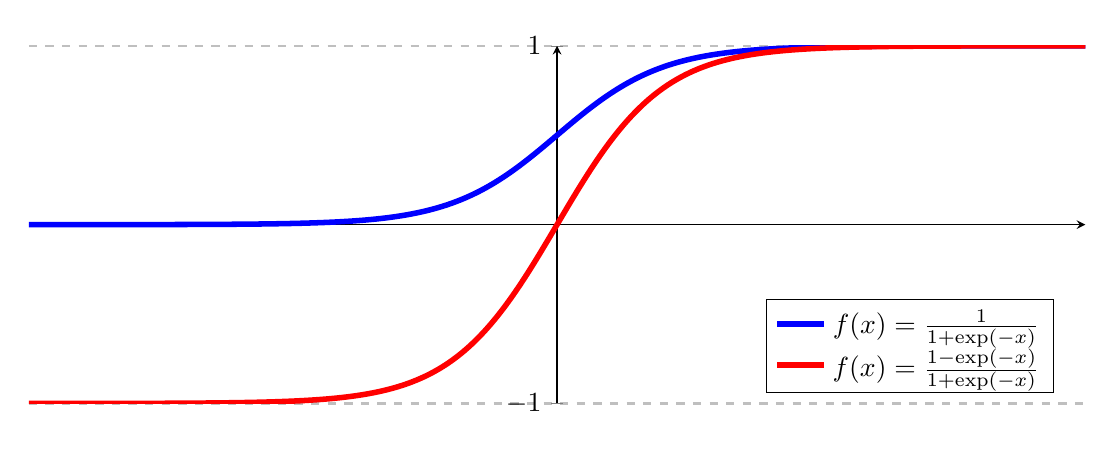
\begin{tikzpicture}
\begin{axis}[ymin=-1, ymax = 1, axis lines = left, legend pos=south east, width=15cm, xmajorticks=false, ytick={-1, +1}, axis lines=middle, y post scale=0.4, ymajorgrids=true, major grid style={dashed, line width=0.8pt}, yticklabel pos=left]
%Here the blue parabloa is defined
\addplot[domain=-10:10, samples=1000, color=blue, line width=2pt]{1/(1 + exp(-x))};
\addplot[domain=-10:10, samples=1000, color=red, line width=2pt]{(1 - e^(-x))/(1 + e^(-x))};
\addlegendentry{$f(x) = \frac{1}{1+\exp(-x)}$}
\addlegendentry{$f(x) = \frac{1 - \exp(-x)}{1 + \exp(-x)}$}
\end{axis}
%\begin{axis}[ymin=-1, ymax = 1, axis lines = left, xlabel = $x$, ylabel = {$f(x)$}]
%%Here the blue parabloa is defined
%\addplot[domain=-10:10, samples=1000, color=red]{(1 - e^(-x))/(1 + e^(-x))};
%\addlegendentry{$(1 - \exp(-x))/(1 + \exp(-x))$}
%\end{axis}
\end{tikzpicture}
% 1/(1+exp(-x))
}
	\caption{Funciones de activación mas utilizadas.}
	\label{fig:funciones}
\end{imagen}


%\subsection{Algoritmo de retropropagación}
El perceptrón multicapa actualiza sus pesos en función de una regla de aprendizaje, de tal manera que los nuevos pesos permitan reducir el error de salida. Por tanto, para cada patrón de entrada a la red es necesario disponer de un patrón de salida deseada. El objetivo es que la salida de la red sea lo más próxima posible a la salida deseada, debido a esto es que el aprendizaje de la red se describe como un problema de minimización de la siguiente manera $$ \min_{W} E $$ donde $W$ es el conjunto de parámetros de la red (pesos y umbrales) y $E$ es una función de error que evalúa la diferencia entre las salidas de la red y las salidas deseadas. En la mayor parte de los casos, la función de error se define como:
\begin{eqnarray}
	E = \frac{1}{N}\sum^{N}_{i = 1} e(i)
\end{eqnarray}

Donde $N$ es el número de muestras y $e(n)$ es el error cometido por la red para el patrón $i$, definido de la siguiente manera
\begin{eqnarray}
	e(i) = \frac{1}{n_{C}}\sum^{n_{C}}_{j = 1} (s_{j}(i) - y^{j}(n))^2\label{eq:error_patron}
\end{eqnarray}

Siendo $Y(i) = (y_{1}(i), y_{2}(i), \cdots, y_{n_{C}}(i))$ y $S(i) = (s_{1}(i), s_{2}(i), \cdots, s_{n_{C}}(i))$ los vectores de salida y salidas deseadas para el patrón $i$ respectivamente.

De esta manera, si $W^{*}$ es un mínimo de la función de error $E$, en dicho punto el error será cercano a cero, y en consecuencia, la salida de la red será próxima a la salida deseada. La presencia de funciones de activación no lineales hace que la respuesta de la red sea no lineal respecto a los parámetros ajustables, por lo que el problema de minimización es un problema no lineal y se hace necesario el uso de técnicas de optimización no lineales para su resolución.

Las técnicas utilizadas suelen basarse en la actualización de los parámetros de la red mediante la determinación de una dirección de búsqueda. En el caso de las redes neuronales multicapa, la dirección de búsqueda más utilizada se basa en la dirección contraria del gradiente de la función de error $E$, el método de gradiente descendente.

Si bien el aprendizaje de la red busca minimizar el error total de la red, el procedimiento está basado en métodos del gradiente estocástico, que son una sucesión de minimizaciones del error $e(i)$ por cada patrón, en lugar de minimizar el error total $E$ de la red. Aplicando el método del gradiente estocástico, cada parámetro $w$ se modifica para cada patrón de entrada $n$ según la siguiente regla de aprendizaje
\begin{eqnarray}
	w(i) = w(n - 1) - \alpha\frac{\partial e(i)}{\partial w}
\end{eqnarray}

donde $e(i)$ es el error para el patrón de entrada $i$ dado por la ecuación \ref{eq:error_patron}, y $\alpha$ es la tasa de aprendizaje, éste último determina el desplazamiento en la superficie del error.

Como las neuronas están ordenadas por capas y en distintos niveles, es posible aplicar el método del gradiente de forma eficiente, resultando en el {\em algoritmo de retropropagación} \cite{Rumelhart1986} o {\em regla delta generalizada}. El término retropropagación es utilizado debido a la forma de implementar el método del gradiente en las redes multicapa, pues el error cometido en la salida de la red es propagado hacia atrás, transformándolo en un error para cada una de las neuronas ocultas de la red.

% Neural Networks for Pattern Recognition - Bishop: 140 - Error backpropagation.
% Neural Networks for Pattern Recognition - Bishop: 263 - Gradient descent.
El algoritmo de retropropagación es el método de entrenamiento más utilizado en redes con conexión hacia adelante. Es un método de aprendizaje supervisado, en el que se distinguen claramente dos fases:
\begin{enumerate}
	\item Se aplica un patrón de entrada, el cual se propaga por las distintas capas que componen la red hasta producir la salida de la misma. Esta salida se compara con la salida deseada y se calcula el error cometido por cada neurona de salida.

	\item Estos errores se transmiten desde la capa de salida, hacia todas neuronas de las capas anteriores \cite{Fritsch1996}. Cada neurona recibe un error que es proporcional a su contribución sobre el error total de la red. Basándose en el error recibido, se ajustan los errores de los pesos sinápticos de cada neurona.
\end{enumerate}








% http://neuralnetworksanddeeplearning.com/chap5.html
% ME ESTOY BASANDO EN : [1998b] Hochreiter
\subsection{El desvanecimiento del gradiente}
El problema del gradiente desvaneciente nace en las NN profundas, éstas utilizan funciones cuyo gradiente se encuentran entre 0 y 1. Debido a que estos gradientes pequeños se multiplican durante la retropropagación, tienden a {\em desvanecerse} a través de las capas, evitando que la red aprenda.

Si se tiene una NN, la activación de una neurona de una capa intermedia $i$ con función de activación $f_i$ y con entrada $$ net_{i}(t) = \sum_{j}w_{ji}y^{j}(t - 1) $$ es $$y^{i}(t) = f_{i}(net_{i}(t))$$ Además $w_{ji}$ es el peso de la conexión desde la unidad $j$ de la capa anterior hasta la unidad $i$ de la capa actual, $d_{k}(t)$ será la respuesta esperada de la unidad $k$ de la capa de salida en el tiempo $t$. Usando el error cuadrático medio ({\em Mean square error}, MSE), el error de $k$ será
$$ E_{k}(t) = (d_{k}(t) - y^{k}(t))^2 $$

En un tiempo $\tau \leq t$ cualquiera, el error de una neurona $j$ que no sea una neurona de entrada es la suma de los errores externos y el error propagado hacia atrás desde la neurona previa será
$$ \vartheta_{j}(\tau) = f'_{j}(net_{j}(\tau))\left(E_{j}(\tau) + \sum_{i} w_{ij}\vartheta_{i}(\tau + 1)\right) $$

El peso actualizado en el tiempo $\tau$ resulta $w_{jl}^{new} = w_{jl}^{old} + \alpha\vartheta_{j}(\tau) y^{l}(\tau - 1)$ donde $\alpha$ es la tasa de aprendizaje, y $l$ es una unidad arbitraria conectada a la unidad $j$.

%\citeA{Puskorius1994}
La propagación hacia atrás de un error que ocurre en una unidad $u$ en un tiempo $t$ hacia una unidad $v$ para $q$ pasos, escala el error de la siguiente manera
\begin{eqnarray}
\frac{\partial\vartheta_{v}(t - q)}{\partial\vartheta_{u}(t)} =
\left\{
\begin{array}{lr}
	f^{'}_{v}(net_{v}(t - 1))w_{uv}	& q = 1\\
	\\
	f^{'}_{v}(net_{v}(t - q))\sum^{n}_{l=1}\frac{\partial\vartheta(t - q + 1)}{\partial\vartheta_{u}(t)}w_{lv}	& q > 1
\end{array}
\right.
\end{eqnarray}

Con $l_{q} = v$ y $l_{0} = u$, el factor de escalamiento es
\begin{eqnarray}
\frac{\partial\vartheta_{v}(t - q)}{\partial\vartheta_{u}(t)} =
\sum^{n}_{l_{1}=1}\cdots\sum^{n}_{l_{q - 1}=1}\prod^{q}_{m = 1}f^{'}_{l_{m}}(net_{l_{m}}(t - m))w_{l_{m}l_{m - 1}}\label{eq:vanishing}
\end{eqnarray}

La sumatoria de los $n^{q - 1}$ términos $\prod^{q}_{m = 1}f^{'}_{l_{m}}(net_{l_{m}}(t - m))w_{l_{m}l_{m - 1}}$ escalan el error. Los distintos términos pueden tener signos diferentes, por lo tanto, el aumento del número de unidades $n$ no implica un incremento del error absoluto. Pero con mas unidades se incrementa la expectativa de que el valor absoluto del error aumente. Si $\rho(m, l_{m}, l_{m - 1}) := |f^{'}_{l_{m}}(net_{l_{m}}(t - m))w_{l_{m}l_{m - 1}}| < 1.0$
para todo $m$, el producto en (\ref{eq:vanishing}) decrece exponencialmente con $q$, es decir, el error se desvanece como muestra la figura \ref{fig:vanishing}. Un error que se desvanece a lo largo del flujo casi no tiene efecto en la actualización de los pesos. %Dada la constante $y^{l_{m - 1}} \neq 0$, $\rho(m, l_{m}, l_{m - 1})$ es máximo cuanto $w_{l_{m}l_{m - 1}} = \frac{1}{y^{l_{m - 1}}}\coth(\frac{net_{l_{m}}}{2})$.

\begin{imagen}
	\scalebox{1.0}{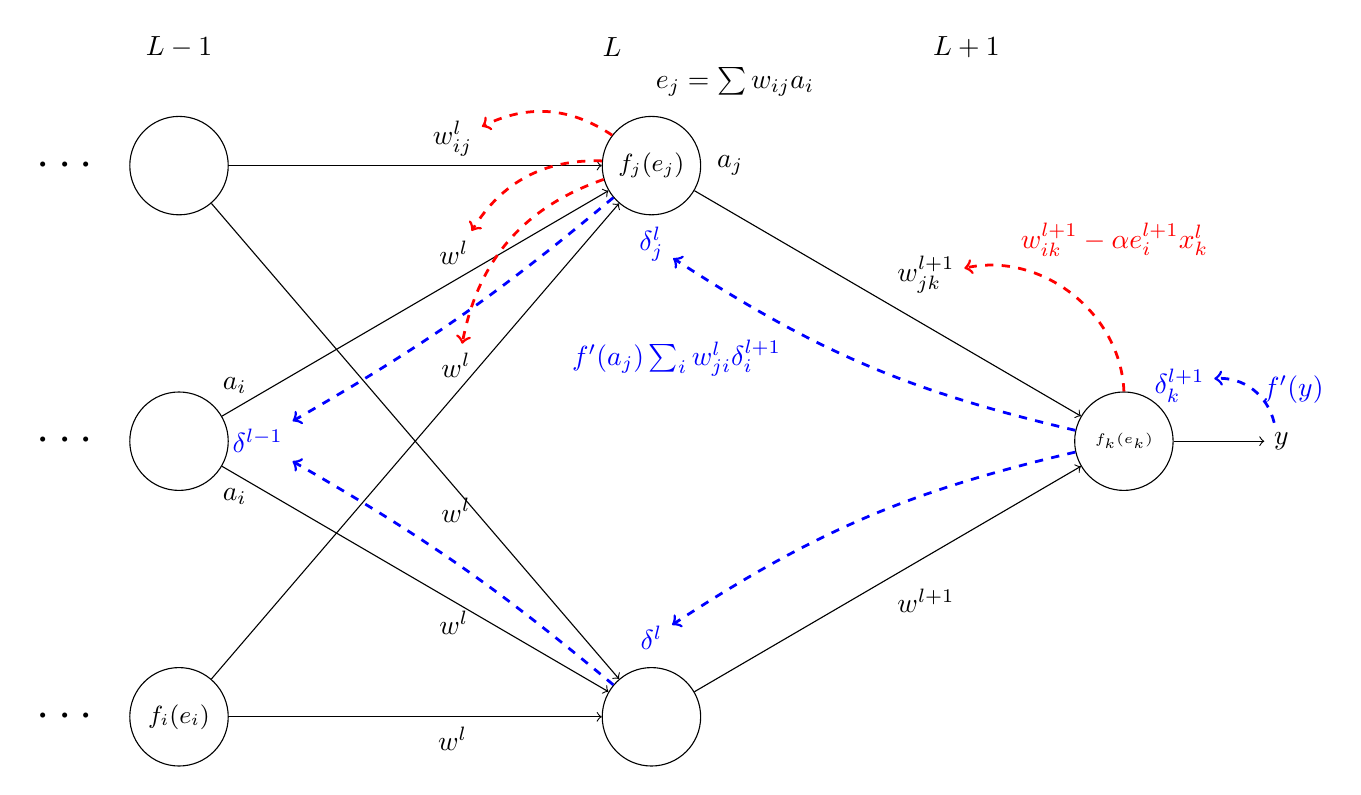
\begin{tikzpicture}

	\tikzstyle{nodo}=[circle, draw, minimum size=1.25cm]
	\tikzstyle{upw}=[dashed, red, ->, line width = 1pt]

	\coordinate (l_0) at (0, 5.0);
	\coordinate (l_1) at (5.5, 5.0);
	\coordinate (l_2) at (10, 5.0);

	\coordinate (f_1_1) at (0, 3.5); % CAPA ENTRADA
	\coordinate (f_1_2) at (0, 0); % CAPA ENTRADA
	\coordinate (f_1_3) at (0, -3.5); % CAPA ENTRADA
	\coordinate (f_2_1) at (6.0, 3.5); % CAPA OCULTA 1
	\coordinate (f_2_2) at (6.0, -3.5); % CAPA OCULTA 1
	\coordinate (f_3_1) at (12, 0); % CAPA SALIDA
	\coordinate (y) at (14, 0); % CAPA SALIDA

	\node[] (l_0) at (l_0) {$L - 1$};
	\node[] (l_1) at (l_1) {$L$};
	\node[] (l_2) at (l_2) {$L + 1$};

	\node[nodo] (f_1_1) at (f_1_1) {}; % CAPA ENTRADA
	\node[nodo] (f_1_2) at (f_1_2) {}; % CAPA ENTRADA
	\node[nodo] (f_1_3) at (f_1_3) {\small $f_i(e_i)$}; % CAPA ENTRADA
	\node[nodo] (f_2_1) at (f_2_1) {\small $f_j(e_j)$}; % CAPA OCULTA 1
	\node[nodo] (f_2_2) at (f_2_2) {}; % CAPA OCULTA 1
	\node[nodo] (f_3_1) at (f_3_1) {\tiny $f_k(e_k)$}; % CAPA SALIDA
	\node[] (y) at (y) {$y$}; % CAPA SALIDA

	\node[left of=f_1_1, node distance=1.4cm] {\LARGE $\cdots$};
	\node[left of=f_1_2, node distance=1.4cm] {\LARGE $\cdots$};
	\node[left of=f_1_3, node distance=1.4cm] {\LARGE $\cdots$};

	\draw[->] (f_1_1) -- node[pos=0.6, above] (w_1_1) {$w^{l}_{ij}$} (f_2_1);
	\draw[->] (f_1_2) -- node[pos=0.6, above] (w_1_2) {$w^{l}_{}$} (f_2_1);
	\draw[->] (f_1_3) -- node[pos=0.6, above] (w_1_3) {$w^{l}_{}$} (f_2_1);
	\draw[->] (f_1_1) node[above right of=f_1_2] {$a_{i}$} -- node[pos=0.6, below] (w_2_1) {$w^{l}_{}$} (f_2_2);
	\draw[->] (f_1_2) node[below right of=f_1_2] {$a_{i}$} -- node[pos=0.6, below] (w_2_2) {$w^{l}_{}$} (f_2_2);
	\draw[->] (f_1_3) -- node[pos=0.6, below] (w_2_3) {$w^{l}_{}$} (f_2_2);
	\draw[->] (f_2_1) node[right of=f_2_1] {$a_{j}$} -- node[pos=0.5, above right] (w_j_k) {$w^{l+1}_{jk}$} (f_3_1);
	\draw[->] (f_2_2) -- node[pos=0.5, below right] {$w^{l+1}$} (f_3_1);
	\draw[->] (f_3_1) -- node[pos=0.5, below right] {$$} (y);

	\node[above right of=f_2_1, node distance=1.5cm] {$e_{j} = \sum w_{ij}a_i$};


	\draw[upw] (f_3_1) to[bend right=50] node[above right, pos=0.8] {$w^{l+1}_{ik} - \alpha e^{l+1}_{i}x^{l}_{k}$} (w_j_k);
	\draw[upw] (f_2_1) to[bend right=30] node[above]{$$} (w_1_1);
	\draw[upw] (f_2_1) to[bend right=30] node[above]{$$} (w_1_2);
	\draw[upw] (f_2_1) to[bend right=30] node[above]{$$} (w_1_3);


	\node[blue, above right of=f_3_1] (e_i) {$\delta^{l+1}_{k}$};
	\node[blue, below of=f_2_1] (e_2_1_i) {$\delta^{l}_{j}$};
	\node[blue, above of=f_2_2] (e_2_2_i) {$\delta^{l}$};
	\node[blue, right of=f_1_2] (e_1_2_i) {$\delta^{l-1}$};

	\draw[upw, blue] (y) to[bend right=40] node[right]{$f'(y)$} (e_i);
	\draw[upw, blue] (f_3_1) to[bend left=10] node[below left, pos=0.7]{$f'(a_{j})\sum_{i}w^{l}_{ji}\delta^{l+1}_{i}$} (e_2_1_i);
	\draw[upw, blue] (f_3_1) to[bend right=10] (e_2_2_i);

	\draw[upw, blue] (f_2_1) to[bend left=5] (e_1_2_i);
	\draw[upw, blue] (f_2_2) to[bend right=5] (e_1_2_i);

\end{tikzpicture}
}
	\label{fig:vanishing}
	\caption{Gradiente descendente}
\end{imagen}

\section{Objetivos del proyecto}
\begin{comment}
En esta sección se presenta el objetivo general y los objetivos específicos de la presente propuesta.
\end{comment}

\subsection{Objetivo general}
Evaluar el desempeño del algoritmo {\em simulated annealing} y su efecto sobre entrenamiento de redes neuronales profundas.


\subsection{Objetivos específicos}
Los objetivos establecidos para el presente trabajo son descritos a continuación
\begin{enumerate}
    \item Definir las reglas de aprendizaje a implementar.
    \item Construir los conjuntos de datos de entrada y salida a analizar.
	\item Establecer los parámetros de las redes neuronales para la experimentación.
	\item Entrenar las redes con los distintos conjuntos de datos.
    \item Establecer las conclusiones del trabajo.
\end{enumerate}

\section{Descripción de la solución}
\begin{comment}
En la presente sección se describe el estado del arte y las características de la solución. Se explicara cual es el propósito de la solución, y posteriormente los alcances y limitaciones establecidas.
\end{comment}

\subsection{Estado del arte}
Describir como solucionan el problema.
\begin{comment}
La más frecuente técnica para inducir cambios rápidos y significativos en la \pam\, ha sido la deflación repentina de los manguitos sobre el muslo \citep{Aaslid1989, Aaslid1991,Lagi1994, Newell1994, Strebel1995, Tiecks1995a}. Con este enfoque, se colocan los manguitos alrededor de ambos muslos y se  genera una presión de \mmhg{20-40} por encima de la presión sistólica durante 2 minutos. Sin embargo, con una autorregulación normal la \cbfv\, vuelve y alcanza su estado basal antes que la \pam. \cite{Aaslid1989} demuestran que la velocidad de recuperación se ve afectada de manera significativa por los niveles de la \pacoo.

%%%%%%%%%%%%%%%%%%%%%%%%%%%%%%%%%%%%%%%%%%%%%%
%%%%%%%% TRANSFER FUNCTION ANALYSIS %%%%%%%%%%
%%%%%%%%%%%%%%%%%%%%%%%%%%%%%%%%%%%%%%%%%%%%%%
La evaluación de la \ca\, mediante el análisis de la función de transferencia está basado en minimizar, en la \ca, el efecto de la oscilación espontánea sobre la \cbfv. El método ha sido extensamente utilizado, por ejemplo, en la investivación del control cardiocasvular, arrítmia sinusal respiratoria y autoregulación renal \citep{Saul1989, Saul1991, Holstein1991}. El análisis espectral, al igual que la transformada rápida de Fourier, transforma la serie en el tiempo de la \bp\, y la \cbfv\, al dominio de la frecuencia. Entonces, la función de transferencia entre las dos señales se calcula como: $$ H(f) = \frac{S_{xy}(f)}{S_{xx}(f)} $$ donde $S_{xx}(f)$ es el autoespectro entre la señal de entrada, \bp, y la de señal de salida, \cbfv \citep{Ainslie2008}. Con la función de potencia relativa asociada (ganancia) y al tiempo (fase) puede ser descrito usando la parte real $H_{R}(f)$ y la parte imaginaria $H_{I}(f)$ de la función de transferencia compleja
\begin{eqnarray}
    \mbox{ganancia : } |H(f)| &=& \sqrt{|H_{R}(f)|^2 + |H_{I}(f)|^2}\\
    \mbox{fase : } \Phi(f) &=& \tan^{-1}\left(\frac{|H_{R}(f)|}{|H_{I}(f)|}\right)
\end{eqnarray}

Una estimación de la fiabilidad de la relación entre las dos señales se puede encontrar como la coherencia cuadrado:
\begin{eqnarray}
    \mbox{coherencia : } MSC(f) &=& \frac{|S_{xy}(f)|^2}{S_{xx}(f)S_{yy}(f)}
\end{eqnarray}
donde $S_{yy}(f)$ es el autoespectro del cambio en la \cbfv.



Como una representación de la relación lineal entre la fluctuación de la presión arterial y el flujo sanguíneo cerebral, la coherencia también se utiliza como una medida de \ca. Una coherencia cercana a cero indica que no hay relación entre la presión arterial y el flujo sanguíneo cerebral, mientras que una coherencia cercana a la unidad sugiere una relación lineal indicando problemas en la \ca.

En los primeros estudios de la \ca\, usando la función de transferencia y la fluctuación espontánea de la \bp, se obtuvieron las estimaciones de la respuesta de la frecuencia de amplitud (ganancia) y la coherencia, pero no la respuesta de frecuencia de fase \citep{Giller1990}.
%%%%%%%%%%%%%%%%%%%%%%%%%%%%%%%%%%%%%%%%%%%%
%%%%%%%%%%%%%%%%%%%%%%%%%%%%%%%%%%%%%%%%%%%%
%%%%%%%%%%%%%%%%%%%%%%%%%%%%%%%%%%%%%%%%%%%%


%%%%%%%%%%%%%%%%%%%%%%%%%%%%%%%%%%%%%%%%%%%%
%%%%%%% VOLTERRA %%%%%%%%%%%%%%%%%%%%%%%%%%%
%%%%%%%%%%%%%%%%%%%%%%%%%%%%%%%%%%%%%%%%%%%%
La presencia de no linealidades en la hemodinámica cerebral se ha sugerido en numerosos estudios \citep{Mitsis2002, Zhang1998, Mitsis2004a, Giller2003}. Por lo tanto, un modelo general de Volterra de dos entradas permitiría describir cuantitativamente los efectos dinámicos de la \abp\, espontánea media y la presión de \etcoo.
%%%%%%%%%%%%%%%%%%%%%%%%%%%%%%%%%%%%%%%%%%%%
%%%%%%%%%%%%%%%%%%%%%%%%%%%%%%%%%%%%%%%%%%%%
%%%%%%%%%%%%%%%%%%%%%%%%%%%%%%%%%%%%%%%%%%%%


%%%%%%%%%%%%%%%%%%%%%%%%%%%%%%%%%%%%%%%%%%%%
%%%%% RECURRENT NEURAL NETWORK %%%%%%%%%%%%%
%%%%%%%%%%%%%%%%%%%%%%%%%%%%%%%%%%%%%%%%%%%%
\cite{Panerai2004} propone las redes neuronales recurrentes con retraso ({\em Time Lagged Recurrent Network}, TLRN) para modelar la relación dinámica entre la \pam\, y la \cbfv. Esta arquitectura particular, representa una visión general para explorar la aplicabilidad de una RNA para el modelamiento de la \cbf, debido a la flexibilidad de utilizar diferentes elementos de proceso ({\em Processing elements}, PE), que contiene información que permite modelar comportamiento dinámico. Memorias a corto plazo de Gamma y Laguerre han sido sugueridos como bloques de construcción para este fin.

La memoria de Laguerre es una combinación en cascada de filtros de paso bajo y paso todo. Las señales basales se obtienen de la convolución de la entrada del filtro de pasa bajo con un conjunto ortogonal de la función de paso todo, por lo cual la correlación de la base es menor que la de una memoria Gamma y la velocidad de adaptación aumenta. Cada filtro de paso todo coloca un cero en el círculo unitario, lo que indica el polo de la etapa anterior. Como resultado, la memoria de Laguerre no atenúa las señales de base.

La arquitectura propuesta por \cite{Panerai2004} posee una memoria Laguerre con tres entradas basales de \abp, una capa oculta con \pe\, no lineales conectados directamente a la \abp\, actual de base, las bases restantes de la memoria Laguerre, y los ciclos de retroalimentación de la memoria \cbfv. Se establece un umbral \pe\, para ajustar la salida. Finalmente, una capa de salida para la \cbfv\, contiene otra memoria Laguerre con tres bases con ciclos de retroalimentación de retardo a la capa oculta \pe.
%%%%%%%%%%%%%%%%%%%%%%%%%%%%%%%%%%%%%%%%%%%%
%%%%%%%%%%%%%%%%%%%%%%%%%%%%%%%%%%%%%%%%%%%%
%%%%%%%%%%%%%%%%%%%%%%%%%%%%%%%%%%%%%%%%%%%%


%%%%%%%%%%%%%%%%%%%%%%%%%%%%%%%%%%%%%%%%%%%%
%%%%% SUPPORT VECTOR MACHINE %%%%%%%%%%%%%%%
%%%%%%%%%%%%%%%%%%%%%%%%%%%%%%%%%%%%%%%%%%%%
\cite{Chacon2011} presenta un modelo basado en $v-SVM$, introducido por \cite{Scholkopf2000}. El algoritmo se basa en el aprendizaje estadístico que funciona como un tubo de radio $\varepsilon$ que encierra a los datos. La frontera de decisión que determina el radio $\varepsilon$ del tubo se obtiene mediante el uso de un subconjunto de ejemplos de entrenamiento llamado Vector de Soporte ({\em Support vector}, \sv). Si $\vec{x}$ representa al vector de datos de entrada, el valor de salida $f(\vec{x})$ está dado por la regresión \svm\, utilizando un vector de pesos $\vec{w}$

Una característica importante de las \svm\, es que ponen énfasis en la distancia de los datos a la línea de regresión utilizando funciones de pérdida, como la función de pérdida $\varepsilon$-sensitiva.

El algoritmo minimiza el riesgo funcional $||\vec{w}||^2$ a la que se añade una penalización dada por las variables de holgura $\xi$ dependiendo de la distancia del dato hasta la línea de regresión.

La variación de la $v-SVM$ de \cite{Scholkopf2000} consiste en agregar $\varepsilon$ al problema de minimización, ponderando por una variable $v$ que ajusta la contribución de $\varepsilon$ entre $0$ y $1$

La solución a este problema de minimización para obtener el vector de peso $\vec{w}$ se encuentra mediante el procedimiento estándar para un problema con restricciones de desigualdad en la aplicación de las condiciones de Kuhn-Tuker al problema dual. La principal ventaja del uso del parámetro $v$ es poder controlar el error y el número de \sv\, con un solo parámetro normalizado.

Para resolver el problema de la regresión no lineal basta con cambiar el producto interno entre dos variables independientes $\vec{x_i}\cdot\vec{x_j}$ por una función Kernel $K(\Phi(\vec{x_i})\cdot\Phi(\vec{x_j}))$. Algunas funciones Kernel que se puede utilizar puede ser la función de base radial gaussiano ($RBF$)
%%%%%%%%%%%%%%%%%%%%%%%%%%%%%%%%%%%%%%%%%%%%
%%%%%%%%%%%%%%%%%%%%%%%%%%%%%%%%%%%%%%%%%%%%
%%%%%%%%%%%%%%%%%%%%%%%%%%%%%%%%%%%%%%%%%%%%
\end{comment}

\subsection{Características de la solución}
La solución propóne un análisis práctico de la convergencia de las redes neuronales profundas mediante la aplicación de la regla de aprendizaje basada en el algoritmo {\em simulated annealing}. El análisis se realizará sobre conjuntos de datos de diferente indole, utilizados en otras investigaciones. Se comparará su desempeño frente a otras reglas de aprendizaje definidas en la literatura.

\subsection{Propósitos de la solución}
El propósito del presente trabajo es analizar la convergencia de las redes neuronales profundas, determinando el comportamiento de diferentes reglas de aprendizaje.

%El propósito del presente trabajo es comparar los resultados del aprendizaje de los métodos dinámicos de la autorregulación cerebral en los seres humanos, determinando las características del proceso en función de las bandas de frecuencias y ruido.

\subsection{Alcances o limitaciones de la solución}
Los alcances y limitaciones descritos para el trabajo son los siguientes
\begin{itemize}
	\item El estudio se plantea desde una perspectiva práctica, precisando conjuntos de datos acotados.

    \item Los datos que se utilizarán son utilizados por \citeA{Morse2016} en su publicación.

	\item Se estudiarán las reglas de aprendizaje definidas por el gradiente estocástico y {\em simulated annealing}.

	\item Las redes neuronales utilizarán la misma configuración para todos los experimentos salvo por la regla de aprendizaje.
\end{itemize}

\section{Metodología, herramientas y ambiente de desarrollo}
A continuación se especifica la metodología, herramientas y ambientes de desarrollo que se utilizarán para llebar a cabo el proyecto.

\subsection{Metodología a usar}
Considerando el aspecto investigativo del trabajo, se considera la utilización del método científico. Entre las actividades que componen la metodología, \citeA{Sampieri2006} describe los siguientes pasos para desarrollar una investigación:

\begin{itemize}
    \item Formulación de la hipótesis: Los modelos lineales y no lineales que aprenden el comportamiento de la autorregulación del flujo sanguíneo cerebral se comportan distinto cuando se utilizan diferentes bandas de frecuencias.

    \item Marco teórico: Una revisión de la literatura donde se aborda el problema planteado, para situarse en el contexto actual de los problemas. Se describirán los modelos que permiten establecer relaciones entre las componentes de la autorregulación cerebral dinámica.

    \item Diseño de la solución: Se deberá diseñar el experimento para generar los modelos y preparar las señales para su evaluación. Diseñar y ejecutar el experimento provocando ruído en las señales utilizadas.

    % \item Análisis y verificación de los resultados: Los resultados se analizarán considerando las estadísticas que ofrece el experimento.
    \item Análisis y verificación de los resultados: Los resultados se analizarán considerando métodos estadísticos con un valor $p < 0.05$ que será considerado como diferencia significativa.

    \item Presentación de los resultados: Se presentarán tablas que describan los resultados obtenidos y que se consideren pertinentes.

    \item Conclusiones obtenidas en el desarrollo de la investigación.
\end{itemize}

\subsection{Herramientas de desarrollo}
Para el desarrollo y ejecución de los experimentos se utilizará un equipo con las siguientes características
\begin{table}[H]
    \centering
    \begin{tabular}{|l|l|}\hline
        Sistema Operativo   & Solus 2017.04.18.0 64-bit\\\hline
        Procesador          & Intel$^\circledR$ Core\texttrademark i5-2450M CPU @ 2.50GHz x 4\\\hline
        RAM                 & 7.7Gb\\\hline
		Gráficos			& Intel$^\circledR$ Sandybridge Mobile\\\hline
        Almacenamiento      & 935,6 GB\\\hline
    \end{tabular}
\end{table}

El software que se utilizará es:
\begin{itemize}
    \item Software: Entorno para computación y gráficos estadísticos R.
    \item Herramienta ofimática: \LaTeX.
\end{itemize}

\subsection{Ambiente de desarrollo}
El desarrollo de la investigación se realizará en el Departamento de Ingeniería Informática de la Universidad de Santiago de Chile, el cual cuenta con una biblioteca y un laboratorio de computación con acceso a internet, para la recopilación de información y para el desarrollo del experimento. Además, se utilizará el hogar del autor, donde se ubica el equipo de desarrollo a utilizar.

\section{Plan de trabajo}
La planificación del trabajo de investigación, se indica en una carta Gantt que se puede apreciar en la Tabla \ref{tab:gantt}, donde se fija como fecha de inicio el día 12 de marzo de 2016 con fecha de término el día 30 de Junio de 2016. En un regimen de trabajo que considera periodos de 5 horas diarias de trabajo promedio, los 7 días de la semana, lo que equivale a un total de 640 horas de trabajo.

\begin{table}[H]
\centering
\caption{Carta Gantt}
\label{tab:gantt}
\scalebox{0.62} {
\begin{tabular}{lllccc}
\hline
%\multicolumn{3}{c}{\textbf{\begin{tabular}[c]{@{}c@{}}NOMBRE DE\\ LA TAREA\end{tabular}}} & \textbf{\begin{tabular}[c]{@{}c@{}}FECHA DE\\ INICIO\end{tabular}} & \textbf{\begin{tabular}[c]{@{}c@{}}FECHA DE\\ TÉRMINO\end{tabular}} & \textbf{\begin{tabular}[c]{@{}c@{}}DURACIÓN\\ (DÍAS)\end{tabular}} \\ \hline
%\multicolumn{3}{l}{PROYECTO DE TESIS}& 07-03-16	&24-06-16	&\\ \hline
					&							&TAREA												& FECHA INICIO		& FECHA TÉRMINO		& DURACIÓN (DÍAS)\\\hline
\multicolumn{3}{l}{PROYECTO DE TESIS}																& 07-03-16				&24-06-16				& --\\ \hline
					& Inicio					&													& 07-03-16				& 08-03-16				& 2\\
					&							& Reunión con el profesor							& 07-03-16				& 07-03-16				& 1\\
					&							& Inscripción del tema								& 08-03-16				& 08-03-16				& 1\\\hline
					& Estado del arte			&													& 09-03-16				& 29-03-16				& 21\\
					&							& Revisión bibliográfica							& 09-03-16				& 18-03-16				& 10\\
					&							& Reunión con el profesor							& 19-03-16				& 19-03-16				& 1\\
					&							& Marco teórico										& 20-03-16				& 29-03-16				& 10\\\hline
					& Desarrollo de la solución	&													& 30-03-16				& 24-04-16				& 26\\
					&							& Análisis											& 30-03-16				& 02-04-16				& 4\\
					&							& Diseño											& 03-04-16				& 06-04-16				& 4\\
					&							& Implementación									& 07-04-16				& 16-04-16				& 10\\
					&							& Pruebas											& 17-04-16				& 19-04-16				& 3\\
					&							& Correcciones										& 20-04-16				& 22-04-16				& 3\\
					&							& Reunión con el profesor							& 23-04-16				& 23-04-16				& 1\\
					&							& Redacción del análisis, diseño e implementación	& 24-04-16				& 24-04-16				& 1\\ \hline
					& Experimentos				&													& 25-04-16				& 25-05-16				& 31\\
					&							& Calibración de parámetros							& 25-04-16				& 29-04-16				& 5\\
					&							& Experimentación									& 30-04-16				& 14-05-16				& 15\\
					&							& Reunión con el profesor							& 15-05-16				& 15-05-16				& 1\\
					&							& Redacción de la experimentación					& 16-05-16				& 25-05-16				& 10\\ \hline
					& Análisis de resultados	&													& 26-05-16				& 08-06-16				& 14\\
					&							& Análisis detallado								& 26-05-16				& 29-05-16				& 4\\
					&							& Interpretación de los resultados					& 30-05-16				& 02-06-16				& 4\\
					&							& Reunión con el profesor							& 03-06-16				& 03-06-16				& 1\\
					&							& Redación de los resultados						& 04-06-16				& 08-06-16				& 5\\ \hline
					& Documento final			&													& 09-06-16				& 24-06-16				& 16\\
					&							& Redacción de la conclusión						& 09-06-16				& 10-06-16				& 2\\
					&							& Revisión del documento							& 11-06-16				& 17-06-16				& 7\\
					&							& Presentación al profesor							& 18-06-16				& 18-06-16				& 1\\ \hline
					& Correcciones				&													& 19-06-16				& 22-06-16				& 4\\
					&							& Versión final										& 23-06-16				& 23-06-16				& 1\\
					&							& Entrega del documento								& 24-06-16				& 24-06-16				& 1\\ \hline
					&							&													& \multicolumn{1}{l}{}	& \multicolumn{1}{l}{}	& \multicolumn{1}{l}{}\\
					&							&													& \multicolumn{1}{l}{}	& \multicolumn{1}{l}{}	& \multicolumn{1}{l}{}
\end{tabular}
}
\end{table}
%\end{comment}

%
%%%%%%%%%%%%%%%%%%%%%%%%%%%%
% Fin cosas importante
%%%%%%%%%%%%%%%%%%%%%%%%%%%


%%%%%%%%%%%%%%%%%%%%%%%%
% Bibliografía
%%%%%%%%%%%%%%%%%%%%%%%%
%\addcontentsline{toc}{section}{Bibliografía}
\newpage
%\bibliografia
\bibliographystyle{apacite}
\bibliography{referencias}
% \bibliographystyle{apa-good}
%%%%%%%%%%%%%%%%%%%%%%%%
% Fin bibliografía
%%%%%%%%%%%%%%%%%%%%%%%%


%%%%%%%%%%%%%%%%%%%%%%%%
% Apéndice
%%%%%%%%%%%%%%%%%%%%%%%%
%
% \appendix
% \clearpage
% \addappheadtotoc
% \appendixpage
%
% \section{Anexo}

%%%%%%%%%%%%%%%%%%%%%%%%
% Fin apéndice
%%%%%%%%%%%%%%%%%%%%%%%%
\end{document}
